
\newcommand{\vecc}[1]{\vec{\mathbf{#1}}}

\subsection{Overview and Domain Reduction}
% Overview
%   - we make a compiler
% for a restricted problem domain
% we generate a large amount of code
% we replace the lambda function with a call to this code
% pure functions with numerical input
% ignore the effects of numerical machine precision
Our solution will be a domain specific compiler that generates code for a conventional compiler e.g. g++ to optimise and turn into machine instructions.
We can define our goals for the compiler as follows:
\begin{itemize}
    \item Supports a large range of problems
    \item Generates code that is faster than the current default code
    \item Provides a user friendly interface for entering problems
    \item Practical to use (e.g. compile times are not too long)
\end{itemize}
To meet these goals it is first important to define the domain in which our compiler operates.

PDEs are mathematical functions.
Hence, we expect that all the substeps of solving PDEs are also mathematical functions.
This is certainly true in the FV scheme.
Looking at our main focus, the patch update step, we can say $\vecc{Q}_{out} = f(\vecc{Q}_{in}, t, dt, \vecc{x}, \vecc{dx})$ where
$\vecc{Q}_{in}$ and $\vecc{Q}_{out}$ are the input and output state of a patch,
$t$ is time,
$dt$ is the time step,
$\vecc{x}, \vecc{dx}$ are vectors describing the current patch's position and size, and $f$ is the patch update function.
Likewise, the numerical method and problem definitions can also be described as mathematical functions. 
Consequently, we can make the assertion that our compiler only needs to support pure functions.
This a useful restriction as it allows us to consider each function isolation, without the complication of side effects.

Our next observation is that mathematical functions accept a fixed length input and produce a fixed length output.
For example if $f$ is defined for $|\vecc{Q}_{in}|=100$ then the behaviour of $f$ on $|\vecc{Q}_{in}|=101$ is undefined.  
This eliminates the possibility of varying length inputs and outputs, again simplifying our compilers domain.
Further to this observation, every input and output is a real number.
We choose this to mean that all inputs and outputs are restricted to \texttt{double}.
This restriction could be relaxed to allow the use of all numerical data types e.g. \texttt{float}, \texttt{int} but will be left inplace to reduce the compiler complexity.

% mby somethingg about how x/3/3/3 == x/3^3

Finally we add the restriction that control flow is not supported.
At first this may appear to be too hash of a restriction which imposes a serious limit on the compilers capabilities.
However, as we will discuss in Section \ref{sec:DAG} a majority, if not all, control flow can be hoisted to DAG (Directed Acyclic Graph) creation as it is not a fundamental feature of the mathematical functions, hence this restriction is a non-issue.
An exception to this are peicewise functions e.g.
\[
    y = \begin{cases} g(x)  & \text{if } x<0.5 \\  h(x)  & \text{if } x\geq 0.5 \\\end{cases}
\]
This will not be supported by the compiler.





\subsection{DAG} \label{sec:DAG}
% What is a DAG - chip model
% [ ] Explain chip model
% [ ] Show example
% [ ] Control flow hoisting

Our compiler will begin with a Directed Acyclic Graph (DAG).
Currently it is the responsibility of a user to create such a DAG, however it would be entirely possible to generate a DAG using a user friendly format such as from a SymPy [REF] formula.
The DAG model we propose takes inspiration from hardware design and languages such a VDHL.

In a hardware design language you define electrical components.
Each component has input and output ports and its output is a function of its input.
Furthermore, it is common place to see specifications and test cases along side a component to be used in verification.

In our DAG every node has a set of input and output ports.
Every input port must receive single value and every output port can transmit a copies of a single value.
Every a node $n$ in our graph can be describes a function: $\vecc{out ports}=n(\vecc{in ports})$ with the number of inputs and outputs being of a fixed length.

A node may be primitive and directly map to a primitive code operation, for example an addition node maps to $out_1 = in_1 + in_2$ (see Figure \ref{fig:bin_add}).
Or a node may be composite, where it is a DAG itself.
Composite nodes would map to functions in the final code output.
Figure \ref{fig:bn} demonstrates composite nodes with the calculation $out_0 = (in_0)^3 + in_1$ where the function \textit{cubed} has been implemented as a subgraph.


\begin{figure}[h!]
    \begin{center}
        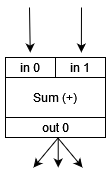
\includegraphics[width=.15\textwidth]{binary_add.png}
        \caption{Example of binary addition as a DAG node.}
        \label{fig:bin_add}
    \end{center}
\end{figure}

\begin{figure}[h!]
    \begin{center}
        \begin{subfigure}{.2\textwidth}
            \begin{center}
                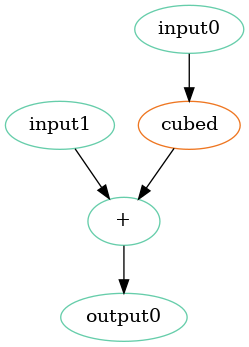
\includegraphics[width=.95\textwidth]{basic-nested-part1.png}
                \caption{Top level}
                \label{fig:bn1}
            \end{center}
        \end{subfigure}%
        \begin{subfigure}{.2\textwidth}
            \begin{center}
                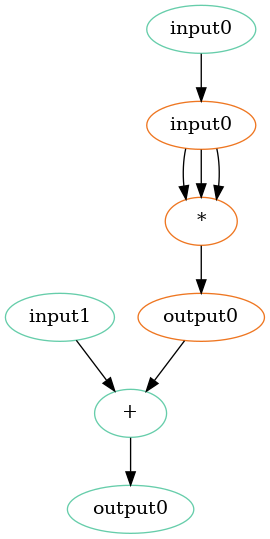
\includegraphics[width=.95\textwidth]{basic-nested-part0.png}
                \caption{Exploded view}
                \label{fig:bn0}
            \end{center}
        \end{subfigure}%
        \caption{Example of a nested DAG that calculates $out_0 = (in_0)^3 + in_1$. NOTE the visualisation displays a node's input edges in a random order.}
        \label{fig:bn}
    \end{center}
\end{figure}


\subsection{IR}
% What is the IR - llvm inspired
% [ ] Explain IR
% [ ] Show example

\subsection{Compiler Architecture}
\subsubsection{Input}
% User provides a DAG

\subsubsection{DAG Transforms}
% [ ] DAG flatten
% 

\subsubsection{DAG to IR}
% DAG -> IR

\subsection{IR Transforms}
% Le none

\subsubsection{Loose IR to Tight IR}
% Loose IR -> Tight IR
%   - variable model
%   - function stencil 


\subsection{Code Generation}
% Tight IR -> Code